% Created by tikzDevice version 0.10.1 on 2018-01-12 16:20:51
% !TEX encoding = UTF-8 Unicode
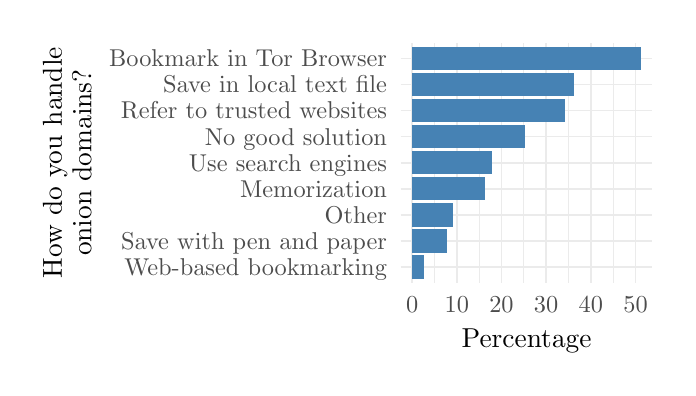
\begin{tikzpicture}[x=1pt,y=1pt]
\definecolor{fillColor}{RGB}{255,255,255}
\path[use as bounding box,fill=fillColor,fill opacity=0.00] (0,0) rectangle (231.26,122.86);
\begin{scope}
\path[clip] (134.78, 30.77) rectangle (225.76,117.36);
\definecolor{drawColor}{gray}{0.92}

\path[draw=drawColor,line width= 0.3pt,line join=round] (146.99, 30.77) --
	(146.99,117.36);

\path[draw=drawColor,line width= 0.3pt,line join=round] (163.13, 30.77) --
	(163.13,117.36);

\path[draw=drawColor,line width= 0.3pt,line join=round] (179.28, 30.77) --
	(179.28,117.36);

\path[draw=drawColor,line width= 0.3pt,line join=round] (195.42, 30.77) --
	(195.42,117.36);

\path[draw=drawColor,line width= 0.3pt,line join=round] (211.57, 30.77) --
	(211.57,117.36);

\path[draw=drawColor,line width= 0.6pt,line join=round] (134.78, 36.42) --
	(225.76, 36.42);

\path[draw=drawColor,line width= 0.6pt,line join=round] (134.78, 45.83) --
	(225.76, 45.83);

\path[draw=drawColor,line width= 0.6pt,line join=round] (134.78, 55.24) --
	(225.76, 55.24);

\path[draw=drawColor,line width= 0.6pt,line join=round] (134.78, 64.65) --
	(225.76, 64.65);

\path[draw=drawColor,line width= 0.6pt,line join=round] (134.78, 74.07) --
	(225.76, 74.07);

\path[draw=drawColor,line width= 0.6pt,line join=round] (134.78, 83.48) --
	(225.76, 83.48);

\path[draw=drawColor,line width= 0.6pt,line join=round] (134.78, 92.89) --
	(225.76, 92.89);

\path[draw=drawColor,line width= 0.6pt,line join=round] (134.78,102.30) --
	(225.76,102.30);

\path[draw=drawColor,line width= 0.6pt,line join=round] (134.78,111.71) --
	(225.76,111.71);

\path[draw=drawColor,line width= 0.6pt,line join=round] (138.91, 30.77) --
	(138.91,117.36);

\path[draw=drawColor,line width= 0.6pt,line join=round] (155.06, 30.77) --
	(155.06,117.36);

\path[draw=drawColor,line width= 0.6pt,line join=round] (171.20, 30.77) --
	(171.20,117.36);

\path[draw=drawColor,line width= 0.6pt,line join=round] (187.35, 30.77) --
	(187.35,117.36);

\path[draw=drawColor,line width= 0.6pt,line join=round] (203.50, 30.77) --
	(203.50,117.36);

\path[draw=drawColor,line width= 0.6pt,line join=round] (219.64, 30.77) --
	(219.64,117.36);
\definecolor{fillColor}{RGB}{70,130,180}

\path[fill=fillColor] (138.91, 32.18) rectangle (143.21, 40.66);

\path[fill=fillColor] (138.91, 41.60) rectangle (151.47, 50.07);

\path[fill=fillColor] (138.91, 51.01) rectangle (153.62, 59.48);

\path[fill=fillColor] (138.91, 60.42) rectangle (165.26, 68.89);

\path[fill=fillColor] (138.91, 69.83) rectangle (167.72, 78.30);

\path[fill=fillColor] (138.91, 79.24) rectangle (179.67, 87.71);

\path[fill=fillColor] (138.91, 88.65) rectangle (194.07, 97.12);

\path[fill=fillColor] (138.91, 98.07) rectangle (197.43,106.54);

\path[fill=fillColor] (138.91,107.48) rectangle (221.63,115.95);
\end{scope}
\begin{scope}
\path[clip] (  0.00,  0.00) rectangle (231.26,122.86);
\definecolor{drawColor}{gray}{0.30}

\node[text=drawColor,anchor=base east,inner sep=0pt, outer sep=0pt, scale=  0.88] at (129.83, 33.39) {Web-based bookmarking};

\node[text=drawColor,anchor=base east,inner sep=0pt, outer sep=0pt, scale=  0.88] at (129.83, 42.80) {Save with pen and paper};

\node[text=drawColor,anchor=base east,inner sep=0pt, outer sep=0pt, scale=  0.88] at (129.83, 52.21) {Other};

\node[text=drawColor,anchor=base east,inner sep=0pt, outer sep=0pt, scale=  0.88] at (129.83, 61.62) {Memorization};

\node[text=drawColor,anchor=base east,inner sep=0pt, outer sep=0pt, scale=  0.88] at (129.83, 71.04) {Use search engines};

\node[text=drawColor,anchor=base east,inner sep=0pt, outer sep=0pt, scale=  0.88] at (129.83, 80.45) {No good solution};

\node[text=drawColor,anchor=base east,inner sep=0pt, outer sep=0pt, scale=  0.88] at (129.83, 89.86) {Refer to trusted websites};

\node[text=drawColor,anchor=base east,inner sep=0pt, outer sep=0pt, scale=  0.88] at (129.83, 99.27) {Save in local text file};

\node[text=drawColor,anchor=base east,inner sep=0pt, outer sep=0pt, scale=  0.88] at (129.83,108.68) {Bookmark in Tor Browser};
\end{scope}
\begin{scope}
\path[clip] (  0.00,  0.00) rectangle (231.26,122.86);
\definecolor{drawColor}{gray}{0.30}

\node[text=drawColor,anchor=base,inner sep=0pt, outer sep=0pt, scale=  0.88] at (138.91, 19.76) {0};

\node[text=drawColor,anchor=base,inner sep=0pt, outer sep=0pt, scale=  0.88] at (155.06, 19.76) {10};

\node[text=drawColor,anchor=base,inner sep=0pt, outer sep=0pt, scale=  0.88] at (171.20, 19.76) {20};

\node[text=drawColor,anchor=base,inner sep=0pt, outer sep=0pt, scale=  0.88] at (187.35, 19.76) {30};

\node[text=drawColor,anchor=base,inner sep=0pt, outer sep=0pt, scale=  0.88] at (203.50, 19.76) {40};

\node[text=drawColor,anchor=base,inner sep=0pt, outer sep=0pt, scale=  0.88] at (219.64, 19.76) {50};
\end{scope}
\begin{scope}
\path[clip] (  0.00,  0.00) rectangle (231.26,122.86);
\definecolor{drawColor}{RGB}{0,0,0}

\node[text=drawColor,anchor=base,inner sep=0pt, outer sep=0pt, scale=  0.99] at (180.27,  7.44) {Percentage};
\end{scope}
\begin{scope}
\path[clip] (  0.00,  0.00) rectangle (231.26,122.86);
\definecolor{drawColor}{RGB}{0,0,0}

\node[text=drawColor,rotate= 90.00,anchor=base,inner sep=0pt, outer sep=0pt, scale=  0.99] at ( 12.32, 74.07) {How do you handle};

\node[text=drawColor,rotate= 90.00,anchor=base,inner sep=0pt, outer sep=0pt, scale=  0.99] at ( 23.01, 74.07) {onion domains?};
\end{scope}
\end{tikzpicture}
